\section{On Risk measures} \label{sec:risk}

When simulating a savings scheme, the first assumption is regarding risk. It is usual to make a stark distinction between risky and risk-free investments. 

But what do we mean by \textit{risk}? We define risk as the uncertainty of the outcome of a given investment. So if we save some money at a $0.1 \%$ bank deposit, we can fairly assume that this investment is risk-free, because we know how much money we will receive at the end. A different scenario could be to invest this money in some market-dependent asset with $1 \%$ expected return but no guarantee of that return. 

But how do we reckon that degree of uncertainty? In stock markets is usual to assume that the price of stocks behaviour is a brownian motion (see~\cite{b:cootner-random, a:samuelson-speculative}), and as such we can define their movement by \textit{trend} and \textit{dispersion} parameters. Since the return obtained by investing in stock assets comes from the relative difference in price between purchase and selling, it is easy to deduce that if we assume that the price follows a geometric brownian motion with trend $\mu$ and dispersion $\sigma$, the expected return of our investment would be $\mu$ with standard deviation $\sigma$. Thanks to this mathematical scheme, we can numerically define the expected return and some degree of uncertainty on it that we will henceforth use as our starting theoretical point. So, the returns at time $t$ are defined as:

\begin{align} \label{eq:return}
    R_t = \frac{P_t - P_{t-1}}{P_{t-1}}\textit{.}
\end{align}

Where $P_t$ is the price of a stock at time $t$ and $P_{t-1}$ is the price of the stock at time $t-1$.

Even though many different models can be assumed to describe the behaviour of the financial markets, the point of this section is to understand and exemplify the set up necessary in order to decide how do we measure risk.

Another way to look at the risk definition is not just looking at dispersion. Using the standard defilogreturnsnition of risk, any unexpected uplift from the expected return would be considered under the umbrella of 'risky outcomes'. Since it is kind of counter-intuitive to assume the probability of a positive outcome as 'risk', it is fair to assume risk as just one half of that dispersion, the negative part of the random variable\footnote{Losses are negative and profits are positive.}.

\begin{figure}
    \centering
    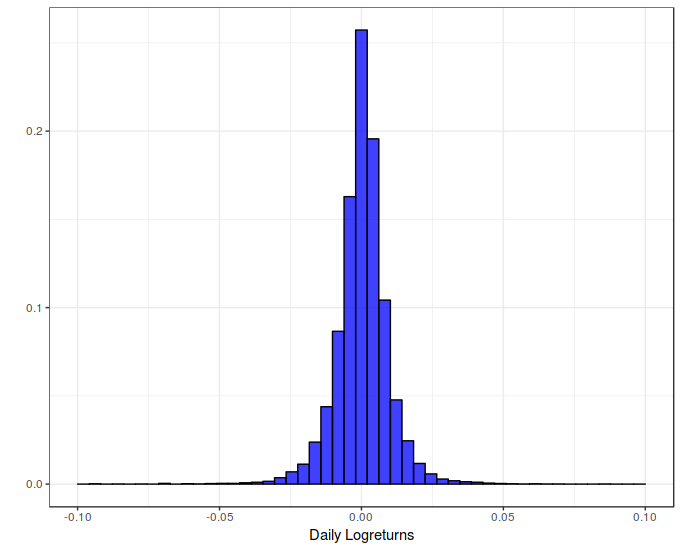
\includegraphics[scale=0.65]{./images/sp_hist.png}
    \caption{Daily logreturns of the Standard \& Poors index [1950 - 2017]. Data from Yahoo Finance.}
    \label{fig:daily-logreturns-sp}
\end{figure}

If we take a look at the actual observed returns in the stock market - as shown in figure~\ref{fig:daily-logreturns-sp} we can see the frequency of different returns. With a little bit of imagination, we can notice a \textit{Bell Curve} shape, and so we could  think of a normal distribution of the logreturns. Where \textit{logreturns} are defined as:

\begin{align} \label{eq:logreturn}
    r_t = \ln{(1+R_t)}\textit{.}
\end{align}

This bell-shaped distribution is important because many financial models assume normality; see Modern Portfolio Theory~\cite{a:markowitz-portfolio}, efficient markets and the Black-Scholes option pricing model. And it is this very normality one of the main assumptions of the geometric brownian motion hypothesis of prices.

But given the irrational and unpredictable behaviour of the markets, we can see some flaws to this normality. Like the fat tails on the extremes of that histogram, fatter than they should, given normality. This little deviation implies that improbable events happen \textit{a lot} more than expected, and this rises a philosophical doubt that undermines our understanding of risk. A normal distribution assumes that, given enough observations, all values in the sample will be distributed equally above and below the mean. Hence the convenience of using standard deviation as a measure of volatility, since it gives us some sense of how far away we can be from the mean. However, given the size of those extreme values, we can not entirely rely our assessment of risk upon the standard deviation; and thus we ought to study and gauge those fat tails further.

\subsection*{Expected Shortfall}

In order to measure the importance and the impact of the tails of return distributions, it is common to compute what is called the \textit{Expected Shortfall}. The Expected Shortfall ($ES_{\alpha}$) at an $\alpha$ quantile of a given distribution $X$ is defined as:

\begin{align} \label{expected-shortfall}
ES_{\alpha} = \frac{1}{\alpha}\int_{0}^{\alpha}VaR_{\gamma}\qty(X)d\gamma \textit{,}
\end{align}

Where $\alpha \in \qty(0,1)$, $VaR_{\gamma}\qty(X)$ is the $1-\gamma$ quantile of $X$ and $\gamma \in \qty(0,1)$. This means that the $ES_{\alpha}$ gives us the expected value of the returns distribution in the worst $\alpha \%$ cases.

Thus, the Expected Shortfall gives us a much more intuitive and reliable sense of the \textit{risk} of any investment; in addition to its useful mathematical properties~\cite{a:bertsimas-shortfall}.

